\titleSlide

\frame{%
    \frametitle{\$::user}
    \framesubtitle{Julien Pivotto}
    \begin{itemize}
        \item{Open-Source consultant at {\inuits{}inuits\small.eu}}
        \item{Puppet User since 2011}
        \item{Speaker/attendee at Puppetcamps}
        \item{Member of the Belgian PUG}
        \item{Puppet core contributor}
        \item{Puppet(labs) modules contributor}
        \olditem{\textit{\ctr{@roidelapluie}} \ctr{on irc/twitter/github}}
    \end{itemize}

}
\inuitsSlide
\picSlideBottom{clabs.png}{%
\begin{center}\LARGE\ctr{http://clusterlabs.org}\end{center}
}
\frame[plain]{%
\centerline{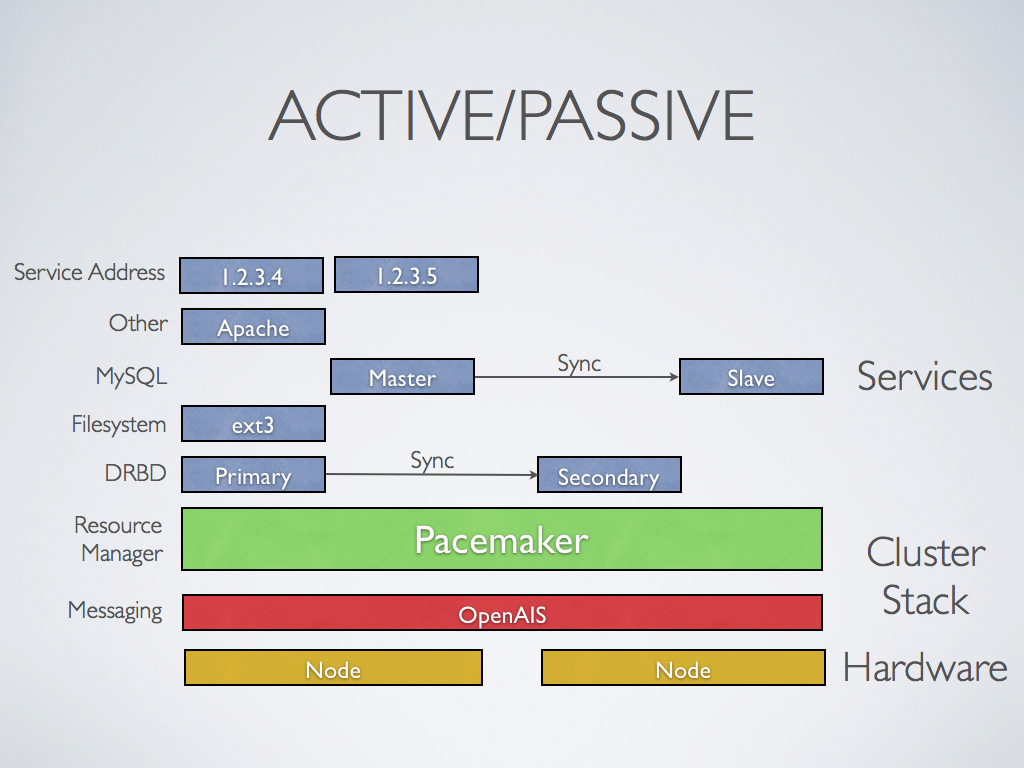
\includegraphics[height=0.9\paperheight]{files/1.png}}\color{grey}http://clusterlabs.org/wiki (GFDL 1.2 licence)
}
\frame[plain]{%
\centerline{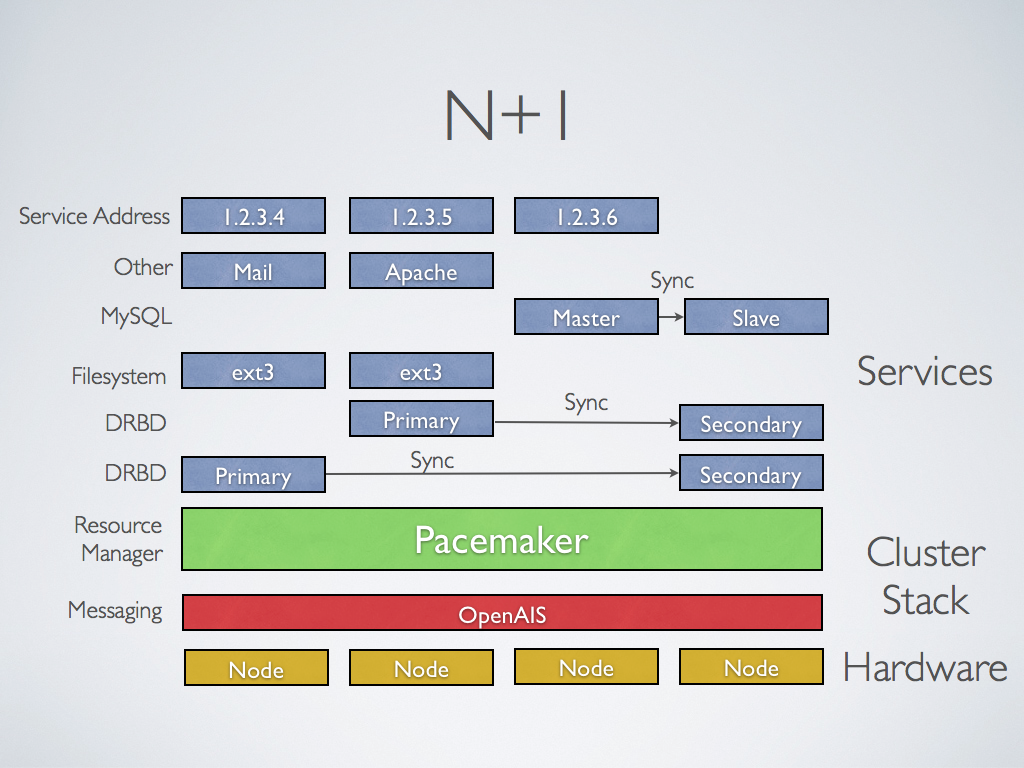
\includegraphics[height=0.9\paperheight]{files/2.png}}\color{grey}http://clusterlabs.org/wiki (GFDL 1.2 licence)
}
\frame[plain]{%
\centerline{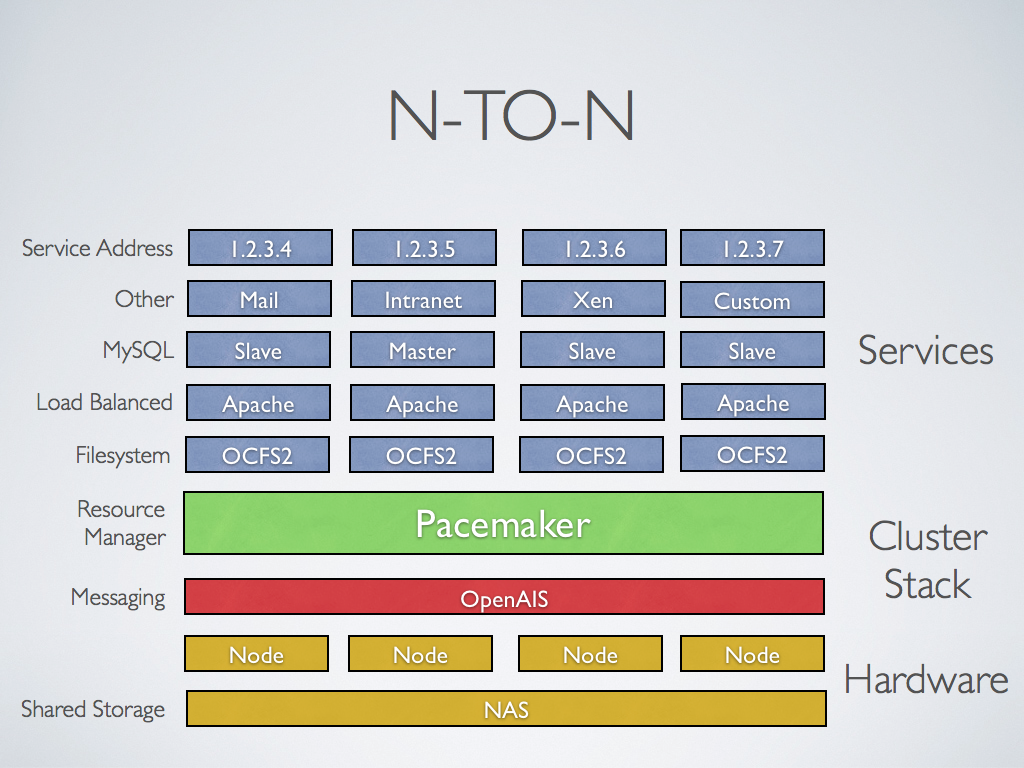
\includegraphics[height=0.9\paperheight]{files/3.png}}\color{grey}http://clusterlabs.org/wiki (GFDL 1.2 licence)
}
\frame[plain]{%
\centerline{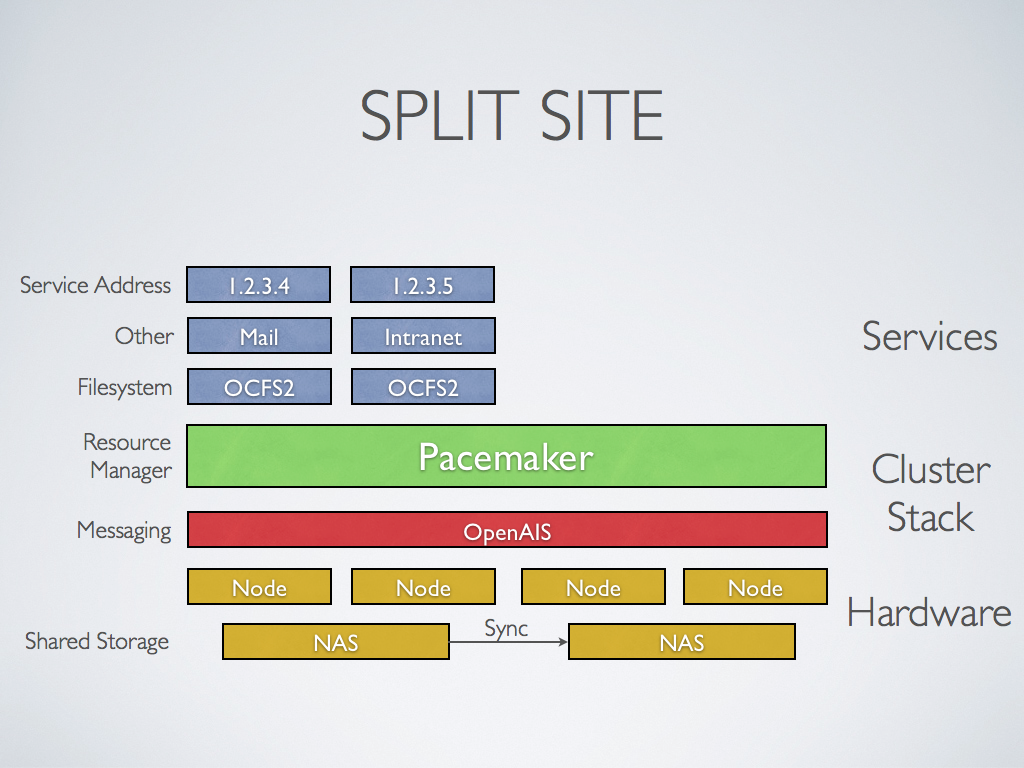
\includegraphics[height=0.9\paperheight]{files/4.png}}\color{grey}http://clusterlabs.org/wiki (GFDL 1.2 licence)
}
\frame{%
    \frametitle{Pacemaker}
    \begin{itemize}
            \item{It is the brain}
        \item{Decides what to do, when}
        \item{Gets information from ressources}
        \item{Depends on messaging \& cluster manager}
        \item{Does not require shared storage}
    \end{itemize}
}
\frame{%
    \frametitle{CIB}
    \begin{itemize}
        \item{Cluster Information Base}
        \item{XML shared accross the cluster}
        \item{Updated using "pcs"}
        \item{Contains knowledge about the cluster}
    \end{itemize}
}

\begin{frame}[fragile]
    \frametitle{Primitives (puppet type)}
    \begin{itemize}
        \item{Service, Ip address, mountpoint,\dots}
        \item{Base bricks of a cluster}
        \item{Get a lot of parameters}
    \end{itemize}
    \begin{verbatim}
primitive ClusterIP ocf:heartbeat:IPaddr2
    params ip="192.168.122.101" cidr_netmask="32"
    op monitor interval="30s"
\end{verbatim}
\end{frame}
\frame{%
    \frametitle{CMAN}
    \begin{itemize}
        \item{Manages membership and quorum}
        \item{EL6 only}
        \item{kbon/puppet-pacemaker}
    \end{itemize}
}
\frame{%
    \frametitle{Corosync}
    \begin{itemize}
            \item{Messaging layer}
            \item{Controlled via CMAN}
        \item{EL6 and EL7: different versions}
        \item{kbon/puppet-cman}
    \end{itemize}
}
\picSlideBottom{pl-forge.png}{}
\picSlideBottom{pl-cs.png}{}
\frame{%

    \frametitle{History}
    \begin{itemize}
        \item{Worked with the "crm" command}
        \item{Which was removed from EL 6.4}
        \item{People got the crm RPM from suse dev}
        \item{RH pushing to use pcs instead}
        \item{jhoblitt integrated pcs in the module}
        \item{I ended that work}
    \end{itemize}

}
\frame{%

    \frametitle{Current Cluster}
    \begin{itemize}
        \item{3 stacks}
        \item{crm+corosync}
        \item{pcs+cman+corosync}
        \item{pcs+corosync}
    \end{itemize}

}
\frame{%

    \frametitle{Current Status}
    \begin{itemize}
        \item{Two providers: pcs crm}
        \item{Bugs bugs bugs}
        \item{Lack of good testing}
        \item{Lack of direction}
    \end{itemize}

}
\frame{%
    \frametitle{Challenges}
    \begin{center}
        \Huge{}\ctr{Pull requests}
    \end{center}
}
\frame{%
    \frametitle{Challenges}
    \begin{center}
        \Huge{}\ctr{EL7}\ctr{Corosync 2}\\\ctr{pcsd}
    \end{center}
}
\frame{%
    \frametitle{Challenges}
    \begin{center}
        \Huge{}\ctr{crm\_shadow}
    \end{center}
}
\frame{%
    \frametitle{Challenges}
    \begin{center}
        \Huge{}\ctr{Testing (beaker?)}
    \end{center}
}
\frame{%
    \frametitle{Conclusion}
    \begin{itemize}
            \olditem{\ctr{I} {\color{red}$\heartsuit$} \ctr{the pacemaker/corosync stack}}
            \olditem{\ctr{I} {\color{red}$\heartsuit$} \ctr{this module}}
            \olditem{\ctr{It needs more} {\color{red}\ctr{$\heartsuit{}\heartsuit{}\heartsuit{}\heartsuit{}$}}}
            \olditem{Give the repo back to community?}
%        \item{I \heartsuit{} this module}
%        \item{It needs more {\heartsuit{}}}
    \end{itemize}
}


\thankyouSlide
\renewcommand{\insertLogo}{}
\contactSlide
